%!TEX encoding = UTF-8 Unicode

%!TEX encoding = UTF-8 Unicode
% coding: utf-8
% Header per le presentazioni in LaTeX+beamer
% @author Eric Miotto
% @date 15/12/2006

\documentclass{beamer}

%Configurazione beamer
\mode<presentation>
{
 %Tema grafico
  \usetheme{Frankfurt}
  
  %Colori da usare per il tema
  \usecolortheme{seahorse} 
  \usecolortheme{rose} 

  \setbeamercovered{transparent}
}

%Importazione package
\usepackage[italian]{babel} %Lingua e sillabazione in italiano
\usepackage[utf8]{inputenc} %Codifica UTF8
\usepackage{textpos} %Posizionamento testo e immagini ovunque sulla pagina

% Griglia di posizionamento delle immagini
% Il primo parametro sono il numero di colonne in cui viene diviso il foglio,
% il secondo sono il numero di righe in cui viene diviso il foglio
%\TPGrid{3}{1}

\title{Presentazione dell'offerta per C04}

\author{Egoless Group}

\date[RR 19/12/2006] % (optional, should be abbreviation of conference name)
{Revisione dei Requisiti, 19 dicembre 2006}

\subject{Presentazione dell'offerta per il capitolato C04}

\logo{
\includegraphics[width=1cm]{img/logo.jpg}}

% Delete this, if you do not want the table of contents to pop up at
% the beginning of each subsection:
\AtBeginSubsection[]
{
  \begin{frame}<beamer>
    \frametitle{Outline}
    \tableofcontents[currentsection,currentsubsection]
  \end{frame}
}

%\AtBeginSection[]
%{
%  \begin{frame}<beamer>
%    \frametitle{Outline}
%    \tableofcontents[currentsection]
%  \end{frame}
%}

\begin{document}

\begin{frame}
  \titlepage
\end{frame}

\begin{frame}
  \frametitle{Outline}
  \tableofcontents
  % You might wish to add the option [pausesections]
\end{frame}


% Structuring a talk is a difficult task and the following structure
% may not be suitable. Here are some rules that apply for this
% solution: 

% - Exactly two or three sections (other than the summary).
% - At *most* three subsections per section.
% - Talk about 30s to 2min per frame. So there should be between about
%   15 and 30 frames, all told.

% - A conference audience is likely to know very little of what you
%   are going to talk about. So *simplify*!
% - In a 20min talk, getting the main ideas across is hard
%   enough. Leave out details, even if it means being less precise than
%   you think necessary.
% - If you omit details that are vital to the proof/implementation,
%   just say so once. Everybody will be happy with that.

\section{Perché abbiamo scelto C04}

\begin{frame}
  \frametitle{Perché abbiamo scelto C04}
  
\begin{itemize}
\item presenza di un proponente tipico
\item interesse nel dominio applicativo
\item presenza \alert{permeante} della qualità
\end{itemize}

\end{frame}

\section{Discussione dell'offerta}

\subsection{Cosa dovrebbe fare il prodotto}

\begin{frame}
  \frametitle{Cosa dovrebbe fare il prodotto}
  \framesubtitle{Riassunto dell'analisi dei requisiti}
  
\begin{itemize}
\item deve supportare le attività della scuola
\item quattro aree principali

\begin{itemize}
\item gestione qualità
\item gestione didattica
\item gestione monitoraggio
\item accesso telematico ai documenti della scuola
\end{itemize}

\begin{center}
  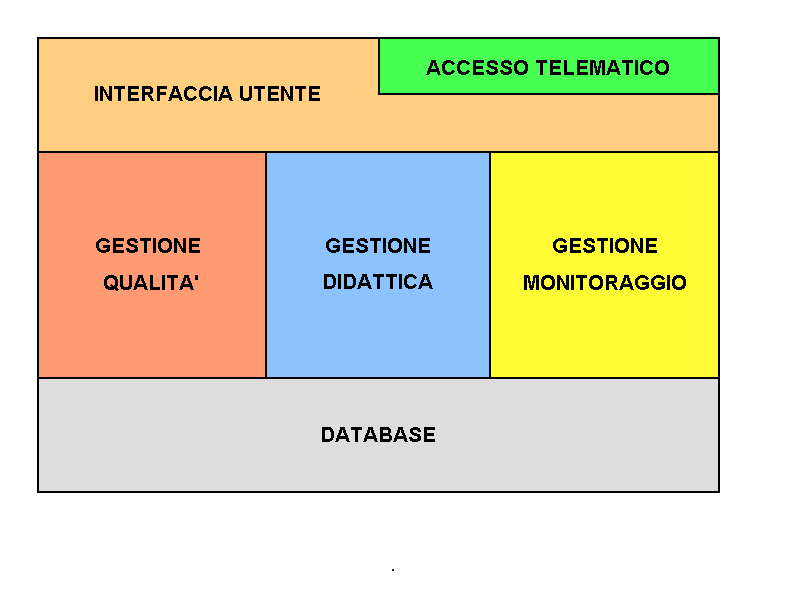
\includegraphics[width=8cm]{img/Sistema.png}
\end{center}

\end{itemize}

\end{frame}

\begin{frame}
\frametitle{Qualità nella scuola}

\begin{itemize}
\item tutto il prodotto è incentrato sulla \alert{qualità}
\item qualità come miglioramento continuo:

\begin{itemize}
\item Plan
\item Do
\item Check
\item Act
\end{itemize}

\end{itemize}

\end{frame}

\begin{frame}
\frametitle{Gestione qualità}

\begin{itemize}
\item aiuta la scuola a pianificare l'attuazione della qualità %diventare conforme ad ISO 9000 e ISO 14000
\item questo si ottiene attraverso gestione dei documenti della qualità
\end{itemize}

\end{frame}

\begin{frame}
\frametitle{Gestione didattica}

\begin{itemize}
\item aiuta concretamente la scuola a svolgere meglio i suoi compiti
\item suddivisa in tre sottoparti
\begin{itemize}
\item gestione studenti
\item gestione professori
\item gestione infrastrutture
\end{itemize}
\end{itemize}

\end{frame}

\begin{frame}
\frametitle{Gestione monitoraggio}

\begin{itemize}
\item rende possibile l'attuazione del miglioramento richiesto dalla qualità
\item tre sottocategorie
\begin{itemize}
\item gestione nonconformità
\item gestione questionari
\item gestione audit
\end{itemize}
\end{itemize}

\end{frame}

\begin{frame}
\frametitle{Accesso telematico ai documenti}

\begin{itemize}
\item migliora e rende trasparenti i rapporti con l'esterno
\item permette l'accesso ad utenti esterni a

\begin{itemize}
\item offerta formativa
\item documenti
\item dati
\end{itemize}

\end{itemize}

\end{frame}

\subsection{Come pensiamo di fare il prodotto}

\begin{frame}
\frametitle{Bisogno guida}

\begin{block}{Bisogno guida}
I gruppi che lavorano su C04 devono produrre complessivamente un solo prodotto.
\end{block}

\begin{itemize}
\item il prof. Zambello desidera ottenere alla fine del corso \alert{un unico prodotto}\ldots
\item \ldots e non $n$ prodotti eterogenei da $n$ gruppi diversi
\end{itemize}

\end{frame}

\begin{frame}
\frametitle{Collaborazione}

\begin{itemize}
\item abbiamo condotto un'analisi dei requisiti che comprende tutto il problema \ldots
\item \ldots poi discuteremo le responsabilità con il prof. Zambello e l'altro gruppo che ha scelto C04 (SWELL System)
\item alla Revisione di Progetto Preliminare raffineremo l'analisi dei requisiti concentrandoci sulla parte che avremo scelto
%\item la nostra ``previsione'': realizzazione gestione didattica
\end{itemize}

\end{frame}

\begin{frame}
\frametitle{Modello di ciclo di vita}

\begin{itemize}
\item abbiamo adottato un \alert{ciclo di vita evolutivo}
\begin{itemize}
\item per gestire lo scenario di collaborazione
\item per affrontare al meglio la nostra inesperienza
\item per gestire la fluidità di fondo dei requisiti
\end{itemize}

\item due iterazioni
\begin{itemize}
\item la prima più lunga per affrontare al meglio i rischi ed evitare di sballare completamente la pianificazione
\item la seconda più corta (sperando di aver appreso qualcosa nella prima\ldots)
\end{itemize}

\end{itemize}

\end{frame}

%\begin{frame}
%\frametitle{La nostra previsione attuale}

%\begin{itemize}
%\item ipotizzando di realizzare tutto il prodotto, si ha la seguente suddivisione:

%\begin{itemize}
%\item prima iterazione: realizzazione gestione didattica, gestione documenti insieme con la parte di autenticazione
%\item seconda iterazione: realizzazione gestione monitoraggio ed accesso telematico
%\end{itemize}
%\item noi naturalmente ci focalizzeremo su una parte del prodotto
%\end{itemize}

%\end{frame}

\subsection{Come pensiamo di fare bene il giusto prodotto}

\begin{frame}
\frametitle{Verifica}

\begin{itemize}
\item la verifica cerca di garantire che i processi producano i risultati attesi nei tempi previsti

\item la verifica opera su

\begin{itemize}
\item fasi dello sviluppo: analisi, progettazione, \ldots
\item documenti: analisi dei requisiti, \ldots
\item prodotto software: codice, \ldots
\end{itemize}

\item la verifica finora è stata rivolta verso i documenti
\end{itemize}


\end{frame}

\begin{frame}
\frametitle{Validazione}

\begin{itemize}
\item la validazione ci assicura che abbiamo fatto il prodotto previsto
\item alpha-test: validazione sui prototipi delle iterazioni
\begin{itemize}
\item tracciamento finale: ulteriore conferma dei tracciamenti fatti nella verifica di ogni fase
\item test per dare prova visibile che i requisiti sono presenti nel software
\end{itemize}

\item beta-test: validazione sul prodotto finale consegnato
\end{itemize}


\end{frame}

\section{Cosa abbiamo sbagliato finora}

\begin{frame}
\frametitle{Cosa abbiamo sbagliato finora}

\begin{itemize}
\item il tempo riservato alla verifica non è stato adeguato
\item inesattezze ed errori rilevati dopo la consegna (sic)
\begin{itemize}
\item discrepanze
\item errori ortografici
\end{itemize}


\item soluzioni
\begin{itemize}
\item documenti già corretti in una versione successiva a quella consegnata
\item stesura di norme che dovrebbero impedire alcuni degli errori
\end{itemize}

\item \alert{altro?}
\end{itemize}

\end{frame}

\end{document}